\documentclass[11pt]{article}
\usepackage{fontspec}
\usepackage[a4paper,margin=2.3cm]{geometry}
\usepackage{graphicx}
\usepackage{booktabs}
\usepackage{array}
\usepackage{xcolor}
\usepackage{float}
\usepackage{fancyvrb}
\usepackage[hidelinks]{hyperref}

\setmainfont{Helvetica Neue}
\setmonofont{Menlo}
\renewcommand{\arraystretch}{1.25}

\title{\textbf{Athena TTS — Clone giọng voiceover}\\[2pt]
\large Nhân bản giọng ``neil'' và nói đúng thoại trong clip ref}
\author{}
\date{15/06/2026}

\begin{document}
\maketitle
\vspace{-1.5em}

\section*{1. Setup}
Dùng một \textbf{giọng voiceover mới} làm mẫu nhân bản, cho 5 engine đọc \textbf{đúng câu
thoại có trong clip ref}, rồi đo độ giống giọng gốc. Chạy CPU (Apple M4 Pro).
\begin{itemize}\setlength\itemsep{1pt}
\item \textbf{Clip ref:} \texttt{refs/neil.wav} (4.5s, trích từ file voiceover \texttt{727407\_\_voiceoverneil}).
\item \textbf{Thoại (transcript clip ref, lấy bằng Whisper):} \texttt{``Ladies and gentlemen, welcome.''}
\item \textbf{Câu cho 5 engine đọc:} đúng câu trên $\Rightarrow$ so sánh ``táo với táo'' cùng nội dung.
\item Bốn engine clone từ \texttt{neil.wav}; Kokoro dùng giọng cài sẵn (không clone) — làm mốc.
\end{itemize}

\section*{2. Cách đo}
Trích \textit{speaker embedding} bằng Resemblyzer (d-vector GE2E), tính \textbf{cosine similarity}
giữa output mỗi engine và clip ref \texttt{neil.wav} (0--1; càng cao càng giống giọng gốc).

\section*{3. Kết quả (cùng câu với clip ref)}
\begin{table}[H]\centering
\begin{tabular}{c >{\bfseries}l r r c}
\toprule
\# & Engine & Cosine $\rightarrow$ neil & Độ dài (s) & Nhân bản giọng \\
\midrule
1 & IndexTTS2  & 0.951 & 3.6 & Có \\
2 & F5-TTS     & 0.876 & 4.0 & Có \\
3 & Chatterbox & 0.873 & 4.0 & Có \\
4 & StyleTTS2  & 0.797 & 3.2 & Có \\
\midrule
-- & Kokoro    & 0.517 & 2.5 & Không (giọng cài sẵn) \\
\bottomrule
\end{tabular}
\end{table}

\begin{figure}[H]\centering
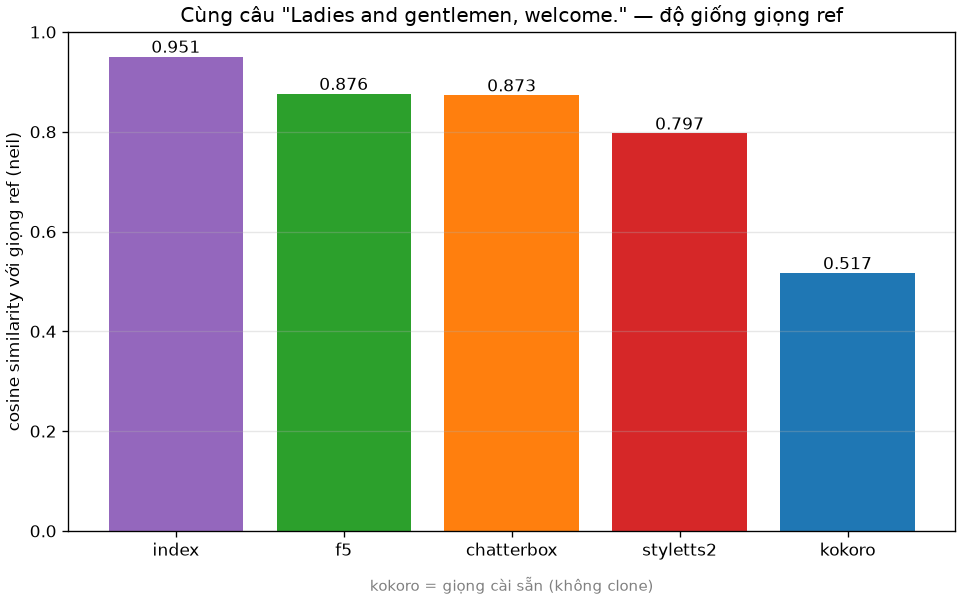
\includegraphics[width=0.82\linewidth]{similarity_refline_chart.png}
\caption{Trục tung: cosine similarity với clip ref neil (0--1). Mỗi cột là một engine.}
\end{figure}

\section*{4. So sánh với câu ngắn khác}
Cùng giọng ref neil, nhưng đọc hai câu khác nhau. Câu càng dài + trùng nội dung clip ref
thì số đo càng ổn định (câu ``See you next time.'' chỉ $\sim$1--2s nên nhiễu hơn).
\begin{table}[H]\centering
\begin{tabular}{>{\bfseries}l r r}
\toprule
Engine & ``See you next time.'' & ``Ladies and gentlemen, welcome.'' \\
\midrule
IndexTTS2  & 0.825 & 0.951 \\
F5-TTS     & 0.801 & 0.876 \\
Chatterbox & 0.699 & 0.873 \\
StyleTTS2  & 0.751 & 0.797 \\
Kokoro     & 0.482 & 0.517 \\
\bottomrule
\end{tabular}
\end{table}

\section*{5. Biểu đồ sóng (cùng câu với clip ref)}
\begin{figure}[H]\centering
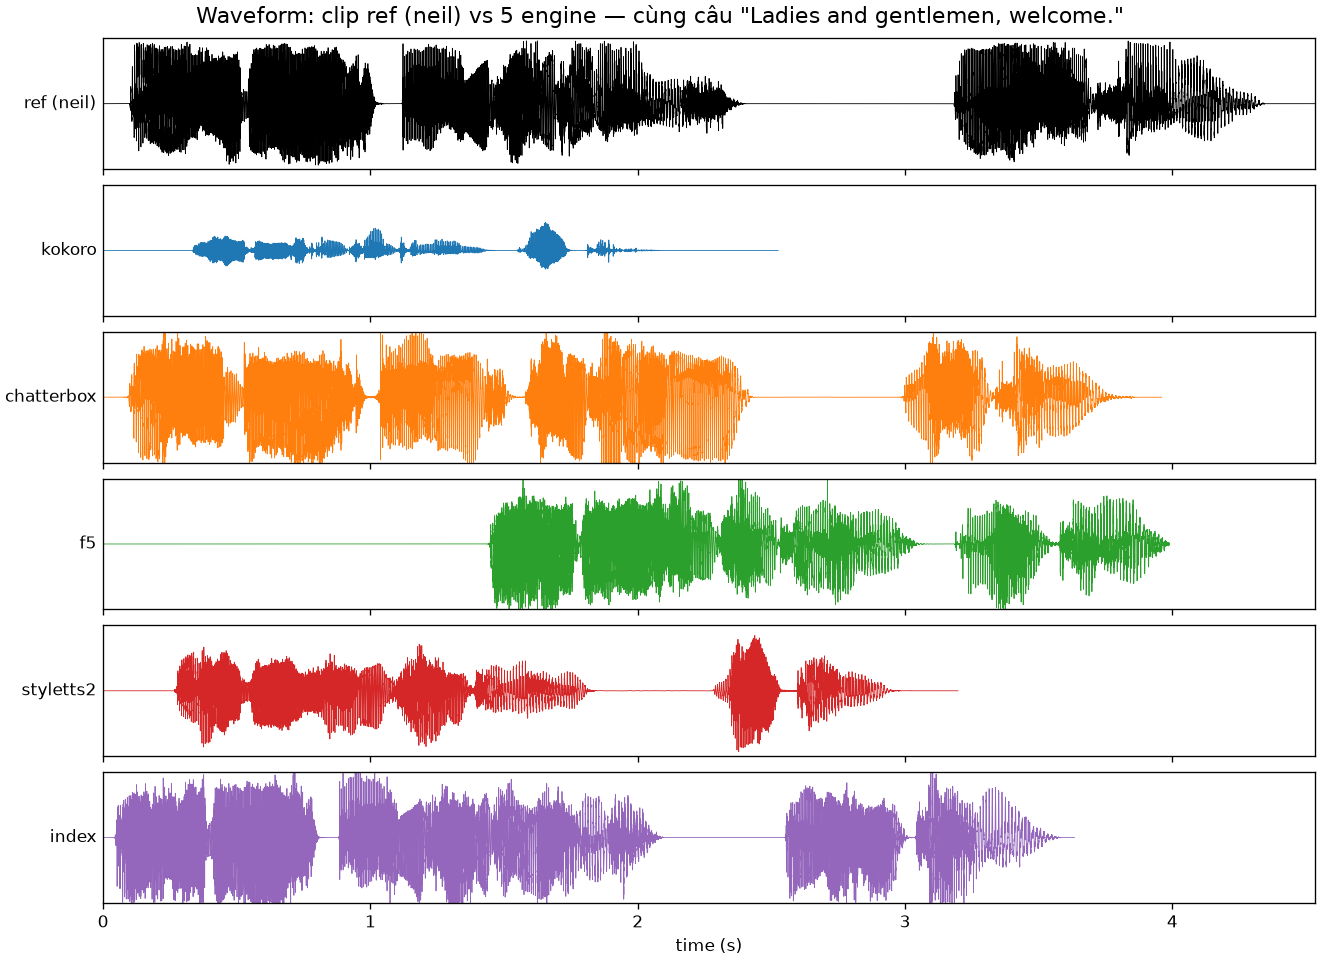
\includegraphics[width=\linewidth]{compare_refline_waveforms.png}
\caption{Trục hoành: thời gian (giây). Trục tung: biên độ tín hiệu (chuẩn hoá $[-1,1]$).
Hàng trên cùng (đen) là clip ref \texttt{neil}; các hàng dưới là 5 engine đọc cùng câu.}
\end{figure}

\end{document}
